\documentclass{report}
\usepackage[utf8]{inputenc}
\usepackage{float}
\usepackage[pdftex]{graphicx}
\usepackage{amsmath}
\usepackage[pdftex]{hyperref}
\DeclareGraphicsExtensions{.pdf,.jpeg,.png,.PNG}

\renewcommand{\figurename}{Imagem}

\title{Construção da Planificação e Levantamento dos Sólidos Platónicos com Transformações Geométricas em 3D}
\author{Pedro Miguel Loureiro Amaral}
\date{20 de Novembro de 2021}

\begin{document}

\maketitle

\renewcommand\thesection{\arabic{section}}

\section{Introdução}

\quad Este relatório tem por objetivo explicar a abordagem e o código desenvolvido para obter uma aplicação em Matlab que mostre, de forma animada, a construção de sólidos platónicos (Cubo, Tetraedro, Octaedro, Icosaedro e Dodecaedro). Para esta construção deverão ser usadas figuras geométricas base regulares (triângulo, quadrado e pentágono). Estas figuras deverão, através de rotações e translações em 2D, formar a planificação de cada sólido e, seguidamente, fixando uma face, as outras deverão sofrer rotações e translações em 3D de modo a "fechar" o sólido. Adicionalmente, as dimensões das figuras devem ser calculadas de modo a que fiquem circunscritas numa circunferência de raio R, definido como argumento do programa.

\section{Organização do Código}

\quad Este projeto segue o paradigma de programação orientada a objetos encontrando-se organizado em classes.

Para representar as figuras foram as desenvolvidas as classes "Triangle", "Square" e "Pentagon". Cada uma destas classes tem os seguintes atributos:
\begin{itemize}
    \setlength\itemsep{0.1em}
    \item initialPoints: contém as coordenadas iniciais dos pontos da figura.
    \item points: contém as coordenadas dos pontos da figura ao longo do programa.
    \item h: "handler" gráfico.
\end{itemize}

As classes das figuras têm também um construtor, que recebe o raio R e uma cor, calcula os pontos iniciais da figura e cria o "handler" gráfico. Adicionalmente, tem os métodos "attach" que será analisado melhor na próxima secção e o método "update" que atualiza a representação gráfica da figura com as novas coordenadas dos pontos.

Para representar os sólidos platónicos foram criadas as classes "Cube", "Tetrahedron", "Octahedron", "Icosahedron" e "Dodecahedron". Cada uma destas classes tem os seguintes atributos:
\begin{itemize}
    \setlength\itemsep{0.1em}
    \item faces: conjunto das figuras pertencentes à planificação do sólido.
    \item size: tamanho de uma aresta.
    \item height: altura de uma figura (apenas para os sólidos contituídos por triângulos ou pentágonos).
    \item width: largura máxima de uma figura (apenas para os sólidos constituídos por pentágonos).
\end{itemize}

As classes dos sólidos têm também um construtor, que recebe o raio R definido pelo utilizador, cria as figuras necessárias para construir o sólido e calcula os restantes atributos. Adicionalmente, tem os seguintes métodos "reset" que restaura as coordenadas atuais dos pontos de todas as figuras às coordenadas iniciais, "update" que atualiza a representação gráfica de todas as figuras com as novas coordenadas dos pontos, "translate" que translaciona todas as faces do sólido ao mesmo tempo segundo os argumentos X, Y e Z e "planificate", "close" e "rotateAroundItself" que serão analisados na próxima secção.

Além das classes referidas anteriormente foram também usadas as funções auxiliares "rotx", "roty" e "rotz" para obter as matrizes de rotação pelo eixo de X, Y e Z e "trans" para obter a matriz de translação.

Por último, a função "Animation" recebe como argumento o raio R que define os tamanhos das figuras e executa a sequência de transformações animadas.

\section{Procedimento}

\subsection{Posicionamento Inicial das Figuras}

\quad As coordenadas iniciais foram definidas de forma a facilitarem as futuras transformações. Assim sendo, todas as figuras têm inicialmente um ponto na origem do referencial facilitando rotações à volta do eixo de Z e uma aresta no eixo de X facilitando rotações sobre a própria aresta.

\begin{figure}[H]
   \centering
   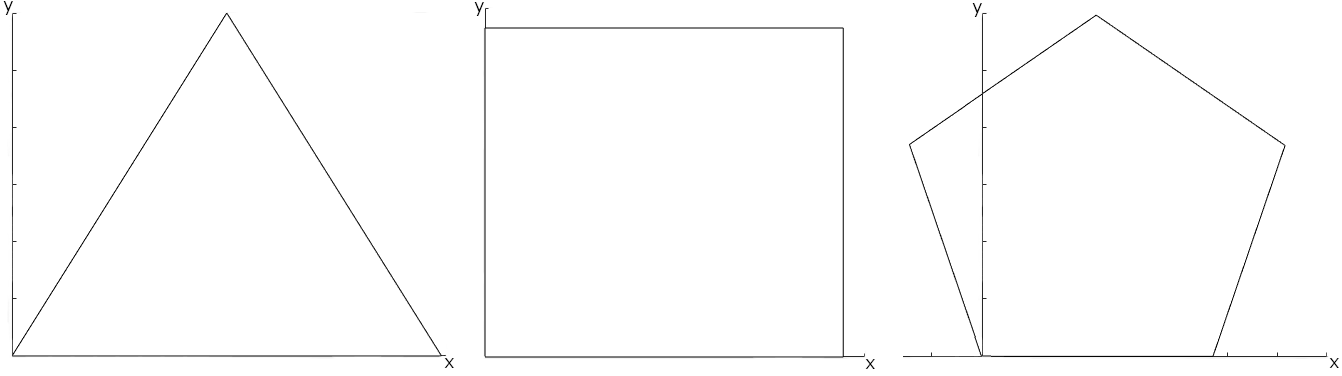
\includegraphics[width=2in]{Figures.PNG}
   \label{fig:figuras}
   \caption{Figuras Base}
\end{figure}

\subsection{Criação da Planificação}

\quad Para a construção da planificação é usado o método "planificate" de cada sólido sendo principalmente usadas translações para a posição necessária. No caso de o sólido necessitar de faces que tenham figuras invertidas, é calculada neste método uma matriz de inversão que corresponde a uma translação para origem seguida de uma rotação em Z seguida de uma translação para aproximadamente a posição onde estava antes. Assim se as figuras necessitarem de ser invertidas, a transformação através da "matriz de inversão" ocorre primeiro e só depois a figura é translacionada para a posição necessária.

\subsection{Levantamento das Faces}

\quad Para "fechar" o sólido é usado o método "close" de cada sólido. Neste método cada figura deve fazer inicialmente uma rotação sobre o eixo de X que, dada a posição inicial da figura, corresponde à rotação sobre a própria aresta. Depois a figura deve efetuar uma rotação à volta do eixo de Z de modo a que essa aresta passe a ser paralela à aresta de uma segunda figura à qual se vai ligar. Por fim, deve efetuar uma translação para que as arestas passem a ser coincidentes. Estas 3 transformações são efetuadas pelo método "attach" presente em cada figura. Após estas transformações, a figura passa a ser considerada como uma extensão da segunda figura e deve repetir todas as transformações que a segunda figura sofre. Para considerar isto no método "attach" existe um argumento opcional "dependentFaces" que se existir é um array de figuras que têm de repetir as transformações. Adicionalmente, para que esta abordagem funcione, o método "attach" só pode ser chamado uma vez para cada face e apenas quando todas as suas faces vizinhas exceto a que a liga à face fixa já o tiverem chamado. Tomando como exemplo a imagem 2, o método attach só pode ser chamado para a face 3 se já tiver sido chamado para a face 4.

\begin{figure}[H]
   \centering
   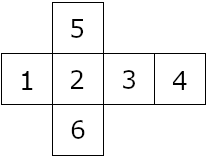
\includegraphics[width=1.3in]{Cube.PNG}
   \label{fig:cubo}
   \caption{Exemplo de planificação}
\end{figure}

\subsection{Rotação de um Sólido sobre Ele Próprio}

\quad Durante a animação de forma a mostrar que o sólido foi construído completamente é necessário mostrar todas as faces usando rotações 3D. Para conseguir rodar um sólido sobre si próprio é usado o método "rotateAroundItself" existente em todas as faces do sólido que calcula o ponto médio todos os pontos de todas as faces do sólido, faz uma translação de forma a que esse ponto médio passe a estar na origem, efetua a rotação em relação ao eixo de Z e depois reverte a translação anterior. Em termos de animação irá ocorrer uma rotação em relação a uma reta paralela ao eixo de Z e à qual o ponto médio pertença.

\subsection{Desmontagem dos Sólidos e das Planificações}

\quad De forma a facilitar a desmontagem dos sólidos e das planificações, os métodos referidos nas últimas subsecções recebem um argumento f que representa fração de progresso nas transformações. Isto faz com que seja possível animar estas transformações mas também possibilita facilmente fazer as transformações inversas bastante progressivamente diminuir a fração em vez de aumentar.

\section{Conclusão}

\quad Concluindo, foram cumpridos todos os requisitos do projeto sendo possível observar na animação a planificação de todos os sólidos e levantamento das faces dos mesmos para os "fechar". Como elemento extra todos os sólidos estão animados em simultâneo e na segunda vez que a planificação e o sólido são construídos na animação eles estão constantemente a rodar sobre si mesmos.

Por fim, segue-se o vídeo demonstrativo: \url{https://youtu.be/j0vQc0xkLk0}.

\end{document}
